% This file was created by tikzplotlib v0.9.8.
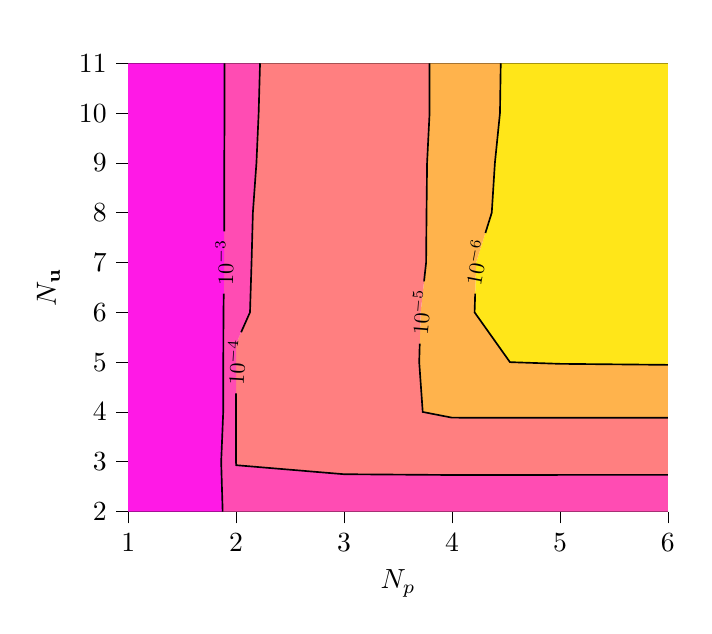
\begin{tikzpicture}

\definecolor{color0}{rgb}{1,0.901960784313726,0.0980392156862745}
\definecolor{color1}{rgb}{1,0.701960784313725,0.298039215686275}
\definecolor{color2}{rgb}{1,0.498039215686275,0.501960784313725}
\definecolor{color3}{rgb}{1,0.298039215686275,0.701960784313725}
\definecolor{color4}{rgb}{1,0.0980392156862745,0.901960784313726}

\begin{axis}[
tick align=outside,
tick pos=left,
%title={Relative Error in Velocity \(\displaystyle \mathbf{u}\) - Max},
title={$\relErrorVelocity$},
x grid style={white!69.0196078431373!black},
xlabel={\(\displaystyle N_p\)},
xmin=1, xmax=6,
xtick style={color=black},
xtick={1,2,3,4,5,6},
xticklabels={
  \(\displaystyle 1\),
  \(\displaystyle 2\),
  \(\displaystyle 3\),
  \(\displaystyle 4\),
  \(\displaystyle 5\),
  \(\displaystyle 6\)
},
y grid style={white!69.0196078431373!black},
ylabel={\(\displaystyle N_{\mathbf{u}}\)},
ymin=2, ymax=11,
ytick style={color=black},
ytick={2,3,4,5,6,7,8,9,10,11},
yticklabels={
  \(\displaystyle 2\),
  \(\displaystyle 3\),
  \(\displaystyle 4\),
  \(\displaystyle 5\),
  \(\displaystyle 6\),
  \(\displaystyle 7\),
  \(\displaystyle 8\),
  \(\displaystyle 9\),
  \(\displaystyle 10\),
  \(\displaystyle 11\)
}
]
\addplot [draw=none, fill=color0]
table{%
x  y
5 4.96599787446714
6 4.94558403088085
6 5
6 6
6 7
6 8
6 9
6 10
6 11
5 11
4.45150563015397 11
4.44439519224548 10
4.39739935034553 9
4.36824322490229 8
4.22374978864749 7
4.20914210167462 6
4.53690125971689 5
5 4.96599787446714
};
\addplot [draw=none, fill=color1]
table{%
x  y
4 3.88534108136274
5 3.883984583036
6 3.88463500185776
6 4
6 4.94558403088085
5 4.96599787446714
4.53690125971689 5
4.20914210167462 6
4.22374978864749 7
4.36824322490229 8
4.39739935034553 9
4.44439519224548 10
4.45150563015397 11
4 11
3.79209881156784 11
3.7920675208487 10
3.76903747323132 9
3.76391793282701 8
3.76005659547684 7
3.70941213226149 6
3.69604662399699 5
3.72869415494111 4
4 3.88534108136274
};
\addplot [draw=none, fill=color2]
table{%
x  y
2 2.93124679617498
3 2.74974998839047
4 2.73430167488701
5 2.73596752053407
6 2.73665469600107
6 3
6 3.88463500185776
5 3.883984583036
4 3.88534108136274
3.72869415494111 4
3.69604662399699 5
3.70941213226149 6
3.76005659547684 7
3.76391793282701 8
3.76903747323132 9
3.7920675208487 10
3.79209881156784 11
3 11
2.22128768144098 11
2.20846393838137 10
2.18801105582443 9
2.15495112430777 8
2.14262579296783 7
2.12827313741416 6
2 5.37581418374384
1.99920268694824 5
1.99894567142086 4
1.99867460329951 3
2 2.93124679617498
};
\addplot [draw=none, fill=color3]
table{%
x  y
2 2
3 2
4 2
5 2
6 2
6 2.73665469600107
5 2.73596752053407
4 2.73430167488701
3 2.74974998839047
2 2.93124679617498
1.99867460329951 3
1.99894567142086 4
1.99920268694824 5
2 5.37581418374384
2.12827313741416 6
2.14262579296783 7
2.15495112430777 8
2.18801105582443 9
2.20846393838137 10
2.22128768144098 11
2 11
1.89268464986793 11
1.89260074197068 10
1.88972363516085 9
1.88904143611823 8
1.88914080571655 7
1.88263020803887 6
1.88085188940186 5
1.8801798059559 4
1.86130344507112 3
1.8749030879246 2
2 2
};
\addplot [draw=none, fill=color4]
table{%
x  y
1.86130344507112 3
1.8801798059559 4
1.88085188940186 5
1.88263020803887 6
1.88914080571655 7
1.88904143611823 8
1.88972363516085 9
1.89260074197068 10
1.89268464986793 11
1 11
1 10
1 9
1 8
1 7
1 6
1 5
1 4
1 3
1 2
1.8749030879246 2
1.86130344507112 3
};
\path [draw=black, semithick]
(axis cs:6,4.94558403088085)
--(axis cs:5,4.96599787446714)
--(axis cs:4.53690125971689,5)
--(axis cs:4.20914210167462,6)
--(axis cs:4.21459959660165,6.37360431786082);

\path [draw=black, semithick]
(axis cs:4.30925730464647,7.59177439623068)
--(axis cs:4.36824322490229,8)
--(axis cs:4.39739935034553,9)
--(axis cs:4.44439519224548,10)
--(axis cs:4.45150563015397,11);

\path [draw=black, semithick]
(axis cs:6,3.88463500185776)
--(axis cs:5,3.883984583036)
--(axis cs:4,3.88534108136274)
--(axis cs:3.72869415494111,4)
--(axis cs:3.69604662399699,5)
--(axis cs:3.70103918778138,5.37354088491024);

\path [draw=black, semithick]
(axis cs:3.74092044627085,6.6221472597187)
--(axis cs:3.76005659547684,7)
--(axis cs:3.76391793282701,8)
--(axis cs:3.76903747323132,9)
--(axis cs:3.7920675208487,10)
--(axis cs:3.79209881156784,11);

\path [draw=black, semithick]
(axis cs:6,2.73665469600107)
--(axis cs:5,2.73596752053407)
--(axis cs:4,2.73430167488701)
--(axis cs:3,2.74974998839047)
--(axis cs:2,2.93124679617498)
--(axis cs:1.99867460329951,3)
--(axis cs:1.99894567142086,4)
--(axis cs:1.9990415933667,4.3732145945417);

\path [draw=black, semithick]
(axis cs:2.04619596162303,5.60060687685705)
--(axis cs:2.12827313741416,6)
--(axis cs:2.14262579296783,7)
--(axis cs:2.15495112430777,8)
--(axis cs:2.18801105582443,9)
--(axis cs:2.20846393838137,10)
--(axis cs:2.22128768144098,11);

\path [draw=black, semithick]
(axis cs:1.8749030879246,2)
--(axis cs:1.86130344507112,3)
--(axis cs:1.8801798059559,4)
--(axis cs:1.88085188940186,5)
--(axis cs:1.88263020803887,6)
--(axis cs:1.88506056188794,6.37329197247242);

\path [draw=black, semithick]
(axis cs:1.88907852229237,7.62678550819736)
--(axis cs:1.88904143611823,8)
--(axis cs:1.88972363516085,9)
--(axis cs:1.89260074197068,10)
--(axis cs:1.89268464986793,11);

\draw (axis cs:4.22374978864749,7) node[
  scale=0.8,
  text=black,
  rotate=79.4
]{$10^{-6}$};
\draw (axis cs:3.70941213226149,6) node[
  scale=0.8,
  text=black,
  rotate=85.6
]{$10^{-5}$};
\draw (axis cs:1.99920268694824,5) node[
  scale=0.8,
  text=black,
  rotate=86.6
]{$10^{-4}$};
\draw (axis cs:1.88914080571655,7) node[
  scale=0.8,
  text=black,
  rotate=89.6
]{$10^{-3}$};
\end{axis}

\end{tikzpicture}
